\section{Perception}
The robot was able to perceive the environment it is situated in using the overhead camera. Using the images provided by the camera, we were able to calculate robot and opponent location and orientation, ball location on the pitch and the pitch itself.

\subsection{Initial approach}
Finding locations of different objects proved to be easy using simple methods like colour segmentation. The main challenge was in calculating robot orientation. Initially we used the dark spot and the T on the plate. This method was not very successful, since isolating the dark spot proved to be hard and inaccurate.
\subsection{Machine Learning}
Later a solution based on Machine-Learning methods was developed. We implemented solutions using SVM and Bayse algorithms available in the OpenCV library. A range of features such as hue moments, compactness and area were used for training a model for each object. We also used distance between two objects, by using this feature we were able to first find a principal object T and then using the distance feature find the correct dark spot close to this object.
\subsection{Central Image Moments}
Even though the Machine-Learning based solution produced reliable outputs but we realised that for a problem of this size, there should be simpler methods available. After studying the literature of computer vision, we implemented a method using second order of central image moments. This method is based on calculating main inertial axes, around which the object can be rotated with minimal or maximal inertia. For detailed description of this method reader is referred to\cite{Teague:80}. Using this method orientation of an object is computed as follows:
\begin{align}
\label{equ:centroid}
\mu'_{20} = \mu_{20} / \mu_{00} = M_{20}/M_{00} - \bar{x}^2 \\
\mu'_{02} = \mu_{02} / \mu_{00} = M_{02}/M_{00} - \bar{y}^2 \\
\mu'_{11} = \mu_{11} / \mu_{00} = M_{11}/M_{00} - \bar{x}\bar{y} \\
\Theta = \frac{1}{2} \arctan2 \left( {2\mu'_{11}},{\mu'_{20} - \mu'_{02}} \right) \label{orientationEq}
\end{align}
One can observe that equation 4 produces results from $-\pi/2$ - $\pi/2$. Our method cannot compute the heading of the calculated vector, to disambiguate this issue we used another method that was developed in earlier stages. It uses central moments of the object and the circle fitted around the object to calculate the orientation\ref{fig:CircleMethod}. This combined solution could produce reliable output. 
\begin{figure}[htp]
\begin{center}
\leavevmode
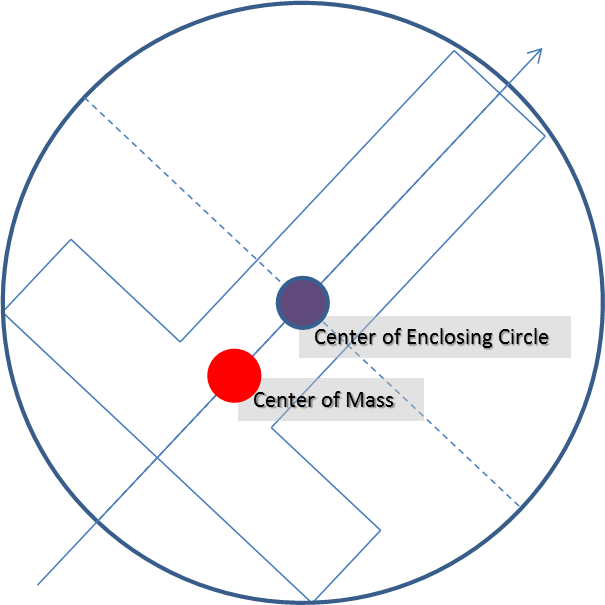
\includegraphics[width=0.2\textwidth] {CenOrien.png}
\end{center}
\caption{Calculating orientation using center of mass of object and surrounding circle, used as a helper for second order of central moments}
\label{fig:CircleMethod}
\end{figure} 
Even though our method calculating robot orientation was not very robust against noise at the specified areas, it was very accurate in 85 to 90\% of the cases. 
\subsection{Results}
Using second order of image moments for calculating orientation of objects was effective for this project. Implementing this method was one of the keys to our success in milestone 3(score 70) and first friendly match(becoming semi-finalist) and later in other
matches. Our initial implementations had a very poor performance of about 5fps, however by the end of the project and using simpler methods we reached frame rates of over 22fps. Our program however suffered from major drops in frame rates on some specific machines in the lab, we could not successfully resolve the issue since the problem was not easily reproducible. This issue was one the major reasons we could not perform very well in the final match. 
A few other achievements in this part of the project was to learn how to effectively use OpenCV library in C. We also learned about Bayes and SVM classifiers and compare their performance.
The developed library contains:
\begin{itemize}
\item Various methods of object isolation methods such as background subtraction and colour segmentation. Various methods of calculating orientation as described earlier.
\item Complete implementation of Machine Learning methods for object recognition.
\item Utility programs for tuning the colour segmentation thresholds.
\item Utility methods for changing functionality of program based on input parameters.
\end{itemize}
\begin{figure}[htp]
\begin{center}
\leavevmode
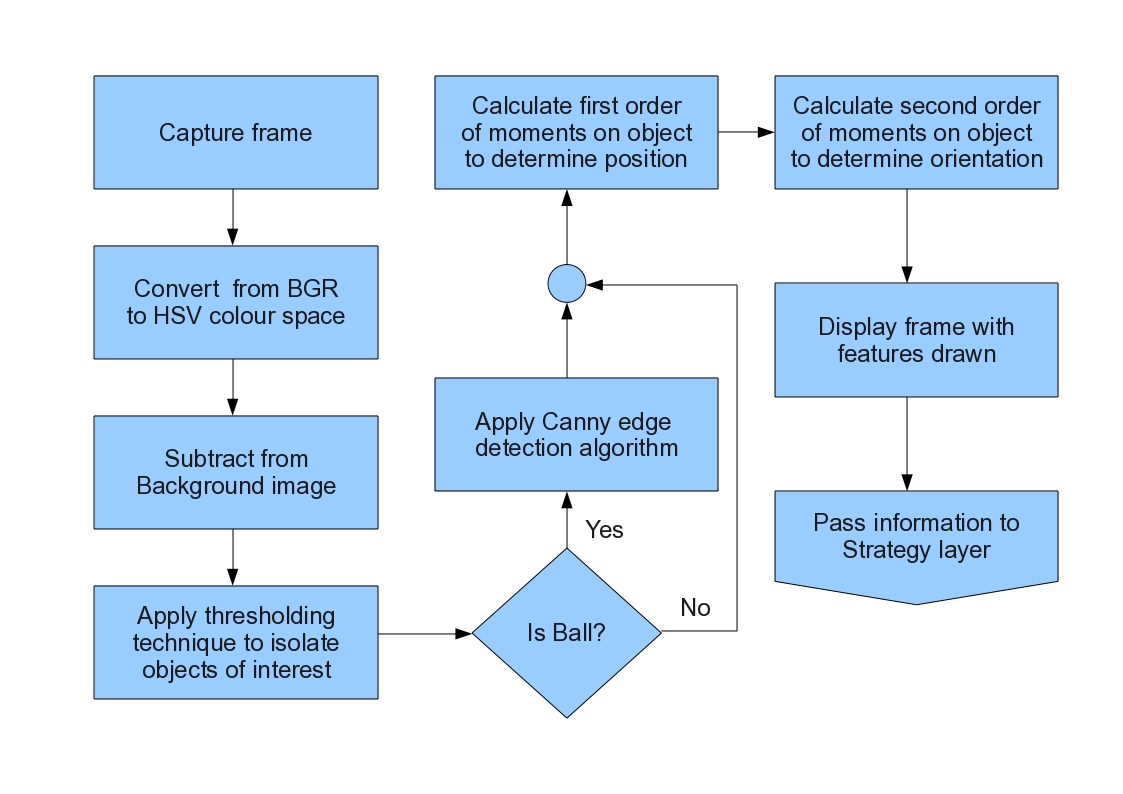
\includegraphics[width=0.4\textwidth] {vision_stack.jpg}
\end{center}
\caption{Final flow chart of vision program}
\label{fig:CircleMethod}
\end{figure}